%% Based on a TeXnicCenter-Template by Gyorgy SZEIDL.
%%%%%%%%%%%%%%%%%%%%%%%%%%%%%%%%%%%%%%%%%%%%%%%%%%%%%%%%%%%%%

%----------------------------------------------------------
%
\documentclass[letterpaper,12pt,openany,reqno]{book}%

%
%----------------------------------------------------------
% This is a sample document for the standard LaTeX Book Class
% Class options
%       --  Body text point size:
%                        10pt (default), 11pt, 12pt
%       --  Paper size:  letterpaper (8.5x11 inch, default)
%                        a4paper, a5paper, b5paper,
%                        legalpaper, executivepaper
%       --  Orientation (portrait is the default):
%                        landscape
%       --  Printside:   oneside, twoside (default)
%       --  Quality:     final(default), draft
%       --  Title page:  titlepage, notitlepage
%       --  Columns:     onecolumn (default), twocolumn
%       --  Start chapter on left:
%                        openright(no, default), openany
%       --  Equation numbering (equation numbers on right is the default):
%                        leqno
%       --  Displayed equations (centered is the default):
%                        fleqn (flush left)
%       --  Open bibliography style (closed bibliography is the default):
%                        openbib
% For instance the command
%          \documentclass[a4paper,12pt,reqno]{book}
% ensures that the paper size is a4, fonts are typeset at the size 12p
% and the equation numbers are on the right side.
%
\usepackage{amsmath}%
\usepackage{amsfonts}%
\usepackage{amssymb}%
\usepackage{graphicx}
\usepackage{tikz}
\usetikzlibrary{shapes,arrows}

\usepackage{float}
\newfloat{mylisting}{thbp}{lob}[chapter]
\floatname{mylisting}{Listing}

\usepackage{listings}
\lstset{ %
xleftmargin={0.5in},						% left margin
language=C,                			% choose the language of the code
columns=flexible,
basicstyle=\small\ttfamily,     % the size of the fonts that are used for the code (was sffamily)
numbers=left,                   % where to put the line-numbers
numberstyle=\small,             % the size of the fonts that are used for the line-numbers
stepnumber=5,                   % the step between two line-numbers. If it's 1 each line will be numbered
numberfirstline=true,						% number the first line of the listing
firstnumber=1,									% auto or <number>
numbersep=5pt,                  % how far the line-numbers are from the code
%backgroundcolor=\color{white},  % choose the background color. You must add \usepackage{color}
showspaces=false,               % show spaces adding particular underscores
showstringspaces=false,         % underline spaces within strings
showtabs=false,                 % show tabs within strings adding particular underscores
frame=single,	                  % adds a frame around the code
tabsize=2,	                    % sets default tabsize to 2 spaces
captionpos=b,                   % sets the caption-position to bottom
breaklines=true,                % sets automatic line breaking
%breakatwhitespace=false,        % sets if automatic breaks should only happen at whitespace
%title=\lstname,                 % show the filename of files included with \lstinputlisting; also try caption instead of title
%escapeinside={\%*}{*)}            % if you want to add a comment within your code
}
\newcommand{\code}[1] {\lstinline[breaklines=yes,breakatwhitespace=yes]{#1}}

%\usepackage[T1]{fontenc}  % access \textquotedbl
%\usepackage{textcomp}     % access \textquotesingle

%---------------------------------------------------
% commands for drawing FAs
\newcommand{\faterminalnode}[3] {\draw (#1) circle [radius=9pt]; \node at (#1) (#2) [circle, draw, minimum size=24pt] {#2};}
\newcommand{\fanonterminalnode}[3] {\node at (#1) (#2) [circle, draw, minimum size=24pt] {#2};}
\newcommand{\fatransition}[3] {\draw [->] (#1) -- (#2) node [midway, above] {#3};}
\newcommand{\faarctransition}[5] {\draw [->] (#1) to[out=#4, in=#5] node  [midway, above] {#3} (#2) ;}
\newcommand{\fastart}[1] {\coordinate (start) at (#1);}
%---------------------------------------------------

\usepackage{mdwlist}
\newenvironment{mydesc}[1][9em]
  {
     \begin{basedescript}
     {
      \renewcommand{\makelabel}[1]{\bfseries##1}
      \desclabelwidth{ #1 }
      \desclabelstyle{\multilinelabel}
     }
  }
  {
     \end{basedescript}%
  }
\makecompactlist{mydesc*}{mydesc}

%----------------------------------------------------------
\newtheorem{theorem}{Theorem}
\newtheorem{acknowledgement}[theorem]{Acknowledgement}
\newtheorem{algorithm}[theorem]{Algorithm}
\newtheorem{axiom}[theorem]{Axiom}
\newtheorem{case}[theorem]{Case}
\newtheorem{claim}[theorem]{Claim}
\newtheorem{conclusion}[theorem]{Conclusion}
\newtheorem{condition}[theorem]{Condition}
\newtheorem{conjecture}[theorem]{Conjecture}
\newtheorem{corollary}[theorem]{Corollary}
\newtheorem{criterion}[theorem]{Criterion}
\newtheorem{definition}[theorem]{Definition}
\newtheorem{example}[theorem]{Example}
\newtheorem{exercise}[theorem]{Exercise}
\newtheorem{lemma}[theorem]{Lemma}
\newtheorem{notation}[theorem]{Notation}
\newtheorem{problem}[theorem]{Problem}
\newtheorem{proposition}[theorem]{Proposition}
\newtheorem{remark}[theorem]{Remark}
\newtheorem{solution}[theorem]{Solution}
\newtheorem{summary}[theorem]{Summary}
\newenvironment{proof}[1][Proof]{\textbf{#1.} }{\ \rule{0.5em}{0.5em}}
%----------------------------------------------------------
\begin{document}

\frontmatter
\title{A Very Simple Compiler Book}
\author{Philip W. Howard}
\date{2019}
\maketitle
\tableofcontents

\chapter{Preface}

Given the existence of other very good books suitable for a course on compilers, why did I choose to write another one? There are several reasons:
  
\begin{enumerate}
\item Most compilers books seem to be written from the perspective that the course is preparing students to actually write a production compiler. That is not the perspective of the compiler courses I've taught. While the students in my course write a complete compiler, I readily acknowledge that very few of my students will work on a compiler as part of their career (although some have). The value of the course has more to do with helping the students to become better developers than in preparing them for a particular field. I have found that this difference in perspective alters what material I find most suitable for the courses I teach. 
\item I find the price of most text books almost criminal. By writing my own text, I can make electronic copies freely available and make printed copies available for a reasonable price.
\end{enumerate}

\mainmatter
%%%%%%%%%%%%%%%%%%%%%%%%%%%%%%%%%%%%%%%%%%%%%%%%%%%%
%% FORMATTING
\setlength{\parindent}{0cm} % Default is 15pt.
\setlength{\parskip}{12pt plus 2pt minus 2pt}
%%%%%%%%%%%%%%%%%%%%%%%%%%%%%%%%%%%%%%%%%%%%%%%%%%%%

\part{Overview}
\chapter{Introduction}
\section{Why?}
The first question that many prospective compiler students have is, ``Why should I study compilers?'' The following answers come to mind:

\begin{enumerate}
\item They're cool. Why wouldn't you want to study compilers?
\item It gives you a chance to understand what your primary tool does. It would seem strange for a carpenter to not know what a hammer does, or to not know the trade-offs between a hammer and a nail gun. Granted, a carpenter doesn't need to know the physics of how these tools work, but they should have a general idea. 

Many software developers never consider their compilers. They have this large blob of software known as an ``IDE''. They type specialized text into their IDE and click various buttons, and if they are luck, they get a working program. My claim is that better programmers have a better understanding of their tools. This allows them to make better use of these tools, and thus better use of their time, and thus (sometimes) more of their employer's money.

\item It gives you a chance to manage a large code base. I've heard of undergraduate computer science students who graduate having never managed anything bigger than a two week lab. In my ten week compiler course, students write an entire compiler composed of tens of source files and thousands of lines of code. Design and implementation decisions made early have strong consequences later in the term. This is a valuable experience that every developer should have before they step into a job claiming they know what they're doing.

Another advantage of the large project is that it allows the introduction of testing techniques that are harder to make ``real'' in smaller environments.

\item Applied data structures. A compiler has a lot of data that needs to be managed. Many data structures present ``clean'' data structures, but real-life data-problems often aren't so clean. How about a cyclic tree that contains links to a stack of hash tables that in turn has links back to nodes of the tree? OK, if your tree is cyclic, you probably have a bug, but most data structures classes don't give you the opportunity to make (and then fix) such bugs. Having the opportunity to get buried in data is good for you.

\item Applied algorithms. I started to learn calculus in high school. I continued my learning of calculus in college. But I didn't really understand what a $dx$ was until I encountered them in my calculus based physics class. They were no longer merely symbols on a paper, they were now applied, and that's how I finally grasped what they really were. In the same sense, a compiler allows you to apply quite a number of algorithms (and data structures). In doing so, they should be more ``real''.

\item Performance considerations. Computers have gotten so fast, we rarely have to worry about performance (time or memory) considerations. Most compiler runs are also fast enough that the compiler's performance doesn't much matter. But given a compiler, you can compile something very big like the Linux Kernel. Performance now matters. Because of this, a compiler class gives the right to talk about performance considerations in a practical sense.

\end{enumerate}

\section{What is a compiler?}
Perhaps before asking, ``Why study compilers?'' it would have been best to establish what a compiler is. But most students, by the time they get to a compiler course, have already used compilers so they have some sense of what they are: The software that translates my source code into executable code. We need to be a bit more formal as well as a bit broader in our definition.

In the broadest sense, a compiler takes code as input and outputs an improved version of that code. For the compiler to be valid, it must follow two guiding principles:
\begin{enumerate}
\item The compiler must preserve the meaning of the original program.
\item The compiler must improve the code in some discernible way.
\end{enumerate}


%----------------------------------------------------------
\begin{figure}[hbt]
\centering
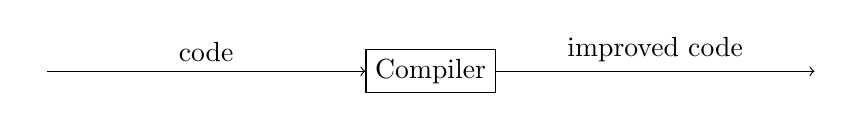
\begin{tikzpicture}
\node (a) at (-5,0) {};
\node (b) at (0,0) [shape=rectangle, draw] {Compiler};
\node (c) at (5,0) {};

\draw [->] (a) -- (b) node [midway, above] {code} ;
\draw [->] (b) -- (c) node [midway, above] {improved code} ;
%\draw [->] (b) -- (c) node [midway, above, text width=3cm, align=center] {improved\\code} ;
\end{tikzpicture}
 \caption[What is a Compiler]{A compiler is a program that takes code as input and outputs an improved version of that code.}
  \label{F.whatiscompiler}
\end{figure}
%----------------------------------------------------------

To illustrate the first principle, if you had a program that output the numbers from $1..10$ and the compiler transformed it so that it output one of e.e. cummings's poems, then clearly the compiler did not preserve the meaning of the original program.

The second principle is a bit less clear. If the code is a program, and you want to execute your program, then transforming your source code into an executable program would be an improvement. But suppose your source was a C program and the output was an equivalent Java program. Would that be an improvement?

This definition of a compiler is deliberately broad. A C preprocessor (often a separate program from the C compiler) is considered a compiler. \LaTeX, which was used to typeset this book, is a compiler. Indeed, any converter program can be considered a compiler given this definition. For the sake of this book (and most compiler courses), we will primarily restrict ourselves to compilers where the input is a programming language. The output, however, does not need to be executable code. It can be any form of ``improved'' coded.

\chapter{Compiler Structure}
Compilers are typically broken into two broad pieces: the front-end and the back-end. The frond-end deals with language specific issues. The back-end deals with target machine specifics.

A C compiler would need a very different front-end compared with a Haskell compiler because the syntax of the languages is very different. One way to view the front-end of the compiler is that it answers the question, ``Is this a valid program?'' If you feed a Scheme program into an R compiler, the answer would certainly by ``No''. If a Java program that was missing a semicolon was fed into a Java compiler, the answer would also be, ``No'', but for very different reasons.

The back-end of a compiler deals with target specific issues. The back-end for a compiler that targets the Java Virtual Machine (JVM) would be different than the back-end for a compiler that targets and ARM processor. Both of those would be different from a C preprocessor that simply outputs text.

Separating the front-end from the back-end makes sense because they are logically quite different, but it also makes sense because if they are properly designed, you can mix and match different front-ends and back-ends. Suppose you had a really good C compiler, but you wanted to port it to target a different machine. There would be no reason to rewrite the front-end. The C language is the same no matter what machine you are targeting. So if you wrote a new back-end and attached it to your existing front-end, you would now have a new compiler. Mixing can go the other way as well. Starting with the same really good C compiler, suppose you wanted a compiler for a different language (such as Go). There is no reason to rewrite the back-end, simply create a front-end for the new language and attach it to your existing back-end, and you have a new compiler.

For this mixing and matching to work seamlessly, there needs to be a common interface between the front-ends and the back-ends. This interface is typically called an Intermediate Representation (IR) --- see Chapter~\ref{chapter.IR}. The front-end translates the language into the IR, and the back-end translates the IR to the target representation. This is illustrated in Figure~\ref{figure.compiler_structure}

%----------------------------------------------------------
\begin{figure}[hbt]
\centering
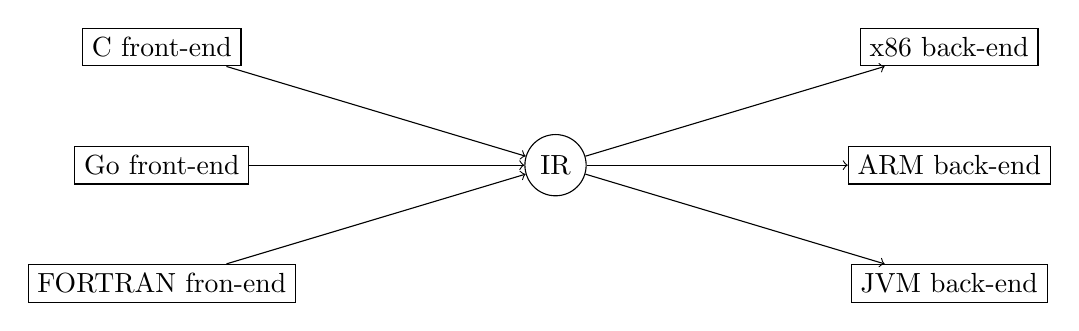
\begin{tikzpicture}
\node (a) at (-5,1.5) [shape=rectangle, draw]{C front-end};
\node (b) at (-5,0) [shape=rectangle, draw] {Go front-end};
\node (c) at (-5,-1.5) [shape=rectangle, draw]{FORTRAN fron-end};
\node (d) at (0,0)  [shape=circle, draw]{IR};
\node (e) at (5,1.5) [shape=rectangle, draw]{x86 back-end};
\node (f) at (5,0) [shape=rectangle, draw] {ARM back-end};
\node (g) at (5,-1.5) [shape=rectangle, draw]{JVM back-end};

\draw [->] (a) -- (d)  ;
\draw [->] (b) -- (d)  ;
\draw [->] (c) -- (d)  ;
\draw [->] (d) -- (e)  ;
\draw [->] (d) -- (f)  ;
\draw [->] (d) -- (g)  ;
\end{tikzpicture}
 \caption[Compiler Structure]{A properly structured compiler allows you to have multiple language-specific front-ends joined to multiple target-specific back-ends. The two a joined using an intermediate representation.}
  \label{figure.compiler_structure}
\end{figure}
%----------------------------------------------------------

Compiler front-ends typically contain two components: A scanner (aka tokenizer or lexer), and a parser. Scanners are discussed in detail in Part~\ref{part.scanner} and parsers are discussed in Part~\ref{part.parser}.

Most computer program source code comes in the form of a stream of characters (a text file). The scanner turns the stream of characters into a stream of tokens. For example, it the scanner read the characters ``\code{some_variable_name}'', it would output the single token \code{IDENTIFIER}. For a longer example, the string ``\code{int main() \{ printf("hello world"\\n); \}}'' would be converted to the tokens ``\code{TYPE IDENTIFIER ( ) \{ IDENTIFIER ( STRING_LIT ) ; \}}''.

Note: Programmers normally format their code to make it ``pretty''. The code in the above examples was not formatted to emphasize that to a compiler, code is just a stream of characters.

The parser takes a stream of tokens and decides whether that stream of tokens makes up a valid program (more specifically a ``compilation unit'') in the language. The parser only looks at the syntax of the language. As a result, ``valid program'' only means ``a program that is syntactically correct''. It does not mean ``a bug free program''.

\chapter{Intermediate Representations} \label{chapter.IR}

\part{Scanning} \label{part.scanner}

\chapter{Regular Expressions}

A scanner turns a stream of characters into a stream of tokens. To facilitate this conversion, most compilers make use of regular expressions to define tokens. Many programmers are familiar with regular expressions from non-compiler contexts. Examples include using an asterisk (*) as a wildcard in a file name, or specifying patterns for the \code{grep} utility. Different programs use different syntax for specifying regular expressions. In this section a minimalist syntax for all regular expressions is presented. Most programs that interpret regular expressions enhance this syntax in various ways to make writing regular expressions easier, but the added syntax does not add extra capabilities.

Regular expressions include the following features:
\begin{mydesc}[10em]
	\item[Concatenation] Concatenation is gluing two strings end-to-end. For example, concatenating ``\texttt{ab}'' with ``\texttt{bc}'' yields the string ``\texttt{abcd}''.
  \item[Alternation] Alternation means to choose exactly one from a set of alternatives. Regular expressions use the vertical bar (\texttt{|}) to mean alternation. So the expression \texttt{a | b | c} means to choose either an '\texttt{a}', a '\texttt{b}', or a '\texttt{c}'.
	\item[Grouping] Parenthesis can be used for grouping operations much as they can in algebraic expressions.
	\item[Kleene Closure] Kleene Closure means to take zero or more instances of a string. Kleene Closure is denoted by an asterisk (\texttt{*}). So, for example, tt{x*} means zero or more '\texttt{x}' characters. Kleene Closure has higher precedence that concatenation so that \texttt{ab*} means \texttt{a(b*)} not \texttt{(ab)*}.
\end{mydesc}

In addition to these operations, the $\Lambda$ symbol is used to represent an empty string (a string with no characters in it).

The most common enhancements to this syntax are as follows:
\begin{mydesc}
\item[zero or one] The question mark (\texttt{?}) indicates zero or one of an item so that \texttt{a?} means the same as \texttt{($\Lambda$ | a)}.
\item[one or more] The plus sign (\texttt{+}) is similar to Kleene Closure, but it is one-or-more not zero-or-more so that \texttt{a+} means the same as \texttt{aa*}.
\item[character range] Square brackets (\texttt{[]}) can be used to specify a character range so that \texttt{[a-m]} means any single character in the range '\texttt{a}' through '\texttt{m}'.
\end{mydesc}

If we want a regular expression for integer constants, we could try
\begin{quote}\texttt{[0-9]+}\end{quote}
but this allows any number of leading zeros. A better expression would be:
\begin{quote}\texttt{[1-9][0-9]*}\end{quote}
This fixes the leading zero problem, but it doesn't allow the number zero. This can be fixed as follows:
\begin{quote}\texttt{0+([1-9][0-9]*)}\end{quote}
If we want to allow negative numbers, we could add an optional minus sign:
\begin{quote}\texttt{0+(-?[1-9][0-9]*)}\end{quote}

\textbf{Exercises}

\begin{enumerate}
\item Write a regular expression for a string containing any odd number of the letter \texttt{a}.
\item Write a regular expression for C (or Java) variable names. Valid characters include upper and lower case letters, digits, and the underscore (\texttt{\_}).
\item Write a regular expression for a string containing any number (including zero) of a positive even number of \texttt{a}'s followed by an add number of \texttt{b}'s. The following are valid strings: \texttt{aaaabbb}, \texttt{aabaabaabbb}, \texttt{aaaaaabbbbbaabaabaab}. The following are not valid strings: \texttt{aaab}, \texttt{aaaabbbaa}, \texttt{bbbaab}.
\item For the previous question, state why each of the non-valid strings are non-valid.
\item Write a regular expression for a floating-point constant. The following rules apply: 
\begin{enumerate}
\item The integer part cannot have leading zeros unless the integer part is zero. 
\item If there is a decimal point, it must be followed by at least one digit.
\item The decimal part must not have trailing zeros unless the decimal part is zero.
\end{enumerate}
\end{enumerate}

\chapter{Creating a Scanner from Regular Expressions}

To specify a scanner for a compiler, a developer could specify a regular expression for each token type. But how do you go from that specification to code that can actually process the input? This chapter discusses the algorithms used to convert regular expressions into a scanner. The general process is to convert the regular expression into a finite automaton. The finite automaton can then be evaluated using a simple table look-up on each character.

\section{Finite Automata}
Finite Automata (aka State Machines) consist of a finite number of states and transitions between states. One state is defined as the start state, and any number of states can be defined as final states. They are often drawn as diagrams as illustrated in Figure~\ref{F.FA_1}.

The start state in an FA is signified by an inbound arrow that doesn't originate from another state. Processing always starts in the start state. Final states are signified by a double circle. Transitions are labeled by the letter that is used to move from one state to another. 

%----------------------------------------------------------
\begin{figure}[hbt]
\centering
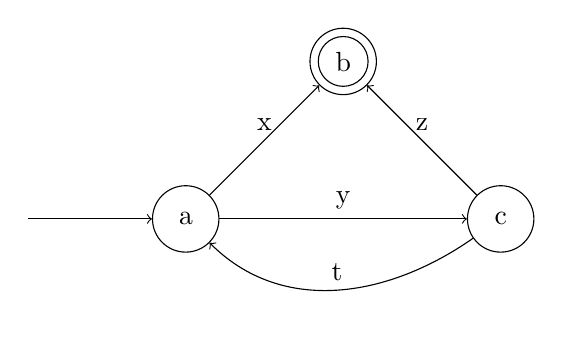
\begin{tikzpicture}

\fastart {-4, -2};
\fanonterminalnode {-2,-2}{a};
\faterminalnode {0,0}{b};
\fanonterminalnode {2,-2}{c};

\fatransition{start}{a}{};
\fatransition{a}{b}{x};
\fatransition{a}{c}{y};
\fatransition{c}{b}{z};
\faarctransition {c}{a}{t}{215}{315};

\end{tikzpicture}
 \caption[Sample Finite Automaton]{This is a sample FA. Node $a$ is the start state (it has an incoming arrow from nowhere). State $b$ is a final state (signified by the double-circle). The transitions are labeled by what letter is used to move from one state to another.}
  \label{F.FA_1}
\end{figure}
%----------------------------------------------------------

Using the FA in Figure~\ref{F.FA_1}, and the input $ytx$, the processing starts in State~$a$ (the start state). The $y$ is used to transition to State~$c$. The $t$ is used to transition back to State~$a$. The $x$ is used to transition to State~$b$. Since the input is exhausted while in a final state, the string is accepted by the FA.

Two conditions can cause a string to be rejected: 
\begin{enumerate}
\item If the input is exhausted and the current state isn't a final state. The input $yty$ illustrates this case.
\item If there is no outbound transition on the current letter. The input $yx$ illustrates this case.
\end{enumerate}

Given these rules from processing FA's, it should be clear that the FA in Figure~\ref{F.FA_1} is equivalent to the regular expression \texttt{(yt)* (x | yz)}

zzz
\section{Thompson's}

This section presents Thompson's construction.

\section{Subset Construction}

This section presents the Subset Construction

\chapter{Scanner Code}
\section{table driven}
Here is a table driven scanner
\section{switch statement}
Here is a table drive scanner

\chapter{Automatically Generated Scanners}
here is a description of flex.

\part{Parsing} \label{part.parser}
\chapter{Context Free Grammars}
\chapter {Top-down recursive-descent parsers}
\chapter {Bottom-up parsers}
\chapter {Automatically generated parsers}
Description of bison.

\part {Semantic Processing}
\chapter {Syntax vs. Semantics}
\chapter {Type systems}
\chapter {Implementation details}

\part{The Back-end}
\chapter {The Visitor Pattern}
\chapter {Code generation}
\chapter {Optimization}

\subsubsection{Subsubsection}

This is just some text under a subsubsection.

\paragraph{Subsubsubsection}

This is just some  text under a subsubsubsection.

\subparagraph{Subsubsubsubsection}

This is just some text under a subsubsubsubsection.


\begin{itemize}
\item Bullet item 1

\item Bullet item 2

\end{itemize}

\begin{description}
\item[Description List] Each description list item has a term followed by the
description of that term.

\item[Bunyip] Mythical beast of Australian Aboriginal legends.
\end{description}

\section{Theorem-Like Environments}

The following theorem-like environments (in alphabetical order) are available
in this style.

\begin{acknowledgement}
This is an acknowledgement
\end{acknowledgement}

\begin{algorithm}
This is an algorithm
\end{algorithm}

\begin{axiom}
This is an axiom
\end{axiom}

\begin{case}
This is a case
\end{case}

\begin{claim}
This is a claim
\end{claim}

\begin{conclusion}
This is a conclusion
\end{conclusion}

\begin{condition}
This is a condition
\end{condition}

\begin{conjecture}
This is a conjecture
\end{conjecture}

\begin{corollary}
This is a corollary
\end{corollary}

\begin{criterion}
This is a criterion
\end{criterion}

\begin{definition}
This is a definition
\end{definition}

\begin{example}
This is an example
\end{example}

\begin{exercise}
This is an exercise
\end{exercise}

\begin{lemma}
This is a lemma
\end{lemma}

\begin{proof}
This is the proof of the lemma.
\end{proof}

\begin{notation}
This is notation
\end{notation}

\begin{problem}
This is a problem
\end{problem}

\begin{proposition}
This is a proposition
\end{proposition}

\begin{remark}
This is a remark
\end{remark}

\begin{summary}
This is a summary
\end{summary}

\begin{theorem}
This is a theorem
\end{theorem}

\begin{proof}
[Proof of the Main Theorem]This is the proof.
\end{proof}

\appendix

\chapter{The First Appendix}

The \verb"\appendix" command should be used only once. Subsequent appendices can
be created using the Chapter command.

\chapter{The Second Appendix}

Some text for the second Appendix.

This text is a sample for a short bibliography. You can cite a book by making use of
the command \verb"\cite{KarelRektorys}": \cite{KarelRektorys}. Papers can be cited
similarly: \cite{Bertoti97}. If you want multiple citations to appear in a single set
of square brackets you must type all of the citation keys inside a single citation,
separating each with a comma. Here is an example: \cite{Bertoti97, Szeidl2001,
Carlson67}.

\begin{thebibliography}{9}
\bibitem {KarelRektorys}Rektorys, K., \textit{Variational methods in Mathematics,
Science and Engineering}, D. Reidel Publishing Company,
Dordrecht-Hollanf/Boston-U.S.A., 2th edition, 1975

\bibitem {Bertoti97} \textsc{Bert\'{o}ti, E.}:\ \textit{On mixed variational formulation
of linear elasticity using nonsymmetric stresses and displacements}, International
Journal for Numerical Methods in Engineering., \textbf{42}, (1997), 561-578.

\bibitem {Szeidl2001} \textsc{Szeidl, G.}:\ \textit{Boundary integral equations for
plane problems in terms of stress functions of order one}, Journal of Computational and
Applied Mechanics, \textbf{2}(2), (2001), 237-261.

\bibitem {Carlson67}  \textsc{Carlson D. E.}:\ \textit{On G\"{u}nther's stress functions
for couple stresses}, Quart. Appl. Math., \textbf{25}, (1967), 139-146.
\end{thebibliography}

\backmatter

\chapter{Afterword}

The back matter often includes one or more of an index, an afterword,
acknowledgements, a bibliography, a colophon, or any other similar item. In
the back matter, chapters do not produce a chapter number, but they are
entered in the table of contents. If you are not using anything in the back
matter, you can delete the back matter TeX field and everything that follows it.
\end{document}
